\documentclass[aspectratio=169,12pt,t]{beamer}

% --- Theme: Metropolis (modern, clean) ---
\usetheme[progressbar=frametitle,numbering=fraction,block=fill]{metropolis}

% --- Fira Sans font (install texlive-fonts-extra if missing) ---
\IfFileExists{FiraSans.sty}{\usepackage[sfdefault]{FiraSans}}{}

% --- Light background with warm accent ---
\definecolor{mDarkTeal}{RGB}{35,55,59}
\definecolor{mLightBrown}{RGB}{235,228,216}
\definecolor{mAccent}{RGB}{140,70,20}

\setbeamercolor{normal text}{fg=mDarkTeal,bg=white}
\setbeamercolor{alerted text}{fg=mAccent}
\setbeamercolor{frametitle}{bg=mDarkTeal,fg=white}
\setbeamercolor{progress bar}{fg=mAccent,bg=mLightBrown}
\setbeamercolor{title separator}{fg=mAccent}
\setbeamercolor{progress bar in head/foot}{fg=mAccent,bg=mLightBrown}
\setbeamercolor{progress bar in section page}{fg=mAccent,bg=mLightBrown}

% --- Packages ---
\usepackage[utf8]{inputenc}
\usepackage{amsmath,amssymb,amsthm}
\usepackage{mathrsfs}
\usepackage{tikz}
\usetikzlibrary{arrows.meta,positioning,calc,decorations.pathreplacing,shapes,patterns}
\usepackage{pgfplots}
\pgfplotsset{compat=1.18}

% --- Semi-transparent white highlight for text on top of background images ---
\usepackage[most]{tcolorbox}

% Inline highlight: \hl{short text}
\newtcbox{\hl}{%
  nobeforeafter, tcbox raise base,
  colback=white, opacityback=0.6,
  colframe=white, opacityframe=0,
  sharp corners, boxsep=2pt, left=3pt, right=3pt, top=2pt, bottom=2pt%
}

% Block highlight: \begin{hlbox} ... \end{hlbox}  (multi-line, paragraphs, itemize)
\newtcolorbox{hlbox}[1][]{%
  enhanced, breakable,
  colback=white, opacityback=0.6,
  colframe=white, opacityframe=0,
  boxsep=3pt, left=6pt, right=6pt, top=4pt, bottom=4pt,
  sharp corners,
  {#1}%
}

% --- Custom colors for content types ---
\definecolor{defcolor}{RGB}{25,85,120}
\definecolor{thmcolor}{RGB}{140,35,35}
\definecolor{proofcolor}{RGB}{35,100,50}
\definecolor{excolor}{RGB}{140,75,10}
\definecolor{remcolor}{RGB}{90,90,90}

% --- Beamer blocks for mathematical content types (semi-transparent) ---
\tcbset{hlblockbase/.style={
  enhanced, breakable,
  coltitle=white, fonttitle=\bfseries,
  opacitybacktitle=0.8, opacityback=0.6,
  opacityframe=0,
  sharp corners,
  boxsep=1pt, left=5pt, right=5pt, top=2pt, bottom=2pt,
  toptitle=1pt, bottomtitle=1pt
}}

\newtcolorbox{defblock}[1]{hlblockbase, title={#1},
  colbacktitle=defcolor, colback=defcolor!15, colframe=defcolor}
\newtcolorbox{thmblock}[1]{hlblockbase, title={#1},
  colbacktitle=thmcolor, colback=thmcolor!15, colframe=thmcolor}
\newtcolorbox{proofblock}[1]{hlblockbase, title={#1},
  colbacktitle=proofcolor, colback=proofcolor!15, colframe=proofcolor}
\newtcolorbox{exblock}[1]{hlblockbase, title={#1},
  colbacktitle=excolor, colback=excolor!15, colframe=excolor}
\newtcolorbox{remblock}[1]{hlblockbase, title={#1},
  colbacktitle=remcolor, colback=remcolor!15, colframe=remcolor}

% --- Metadata ---
\title{Chapter 3: Numerical Sequences and Series}
\subtitle{Section: Upper and Lower Limits}
\author{Based on Walter Rudin's \emph{Principles of Mathematical Analysis}}
\date{}

\begin{document}

% =============================================================================
% TITLE AND OUTLINE
% =============================================================================
{
\usebackgroundtemplate{%
  
\includegraphics[width=\paperwidth,height=\paperheight,keepaspectratio=false]{chapter_03_bg_00.png}%
}
\begin{frame}[plain]
  \titlepage
  \note{
    Welcome back to Chapter 3 of Principles of Mathematical Analysis.
    So far we have studied convergent sequences, subsequences, and
    Cauchy sequences. In this section we broaden our vocabulary to
    handle sequences that may fail to converge. We first define what
    it means for a sequence to diverge to plus or minus infinity, and
    then we introduce two robust quantities, the upper and lower
    limits, which always exist in the extended real line. They will
    let us speak meaningfully about the asymptotic ceiling and floor
    of any real sequence, convergent or not.
  }
\end{frame}
}

{
\usebackgroundtemplate{%
  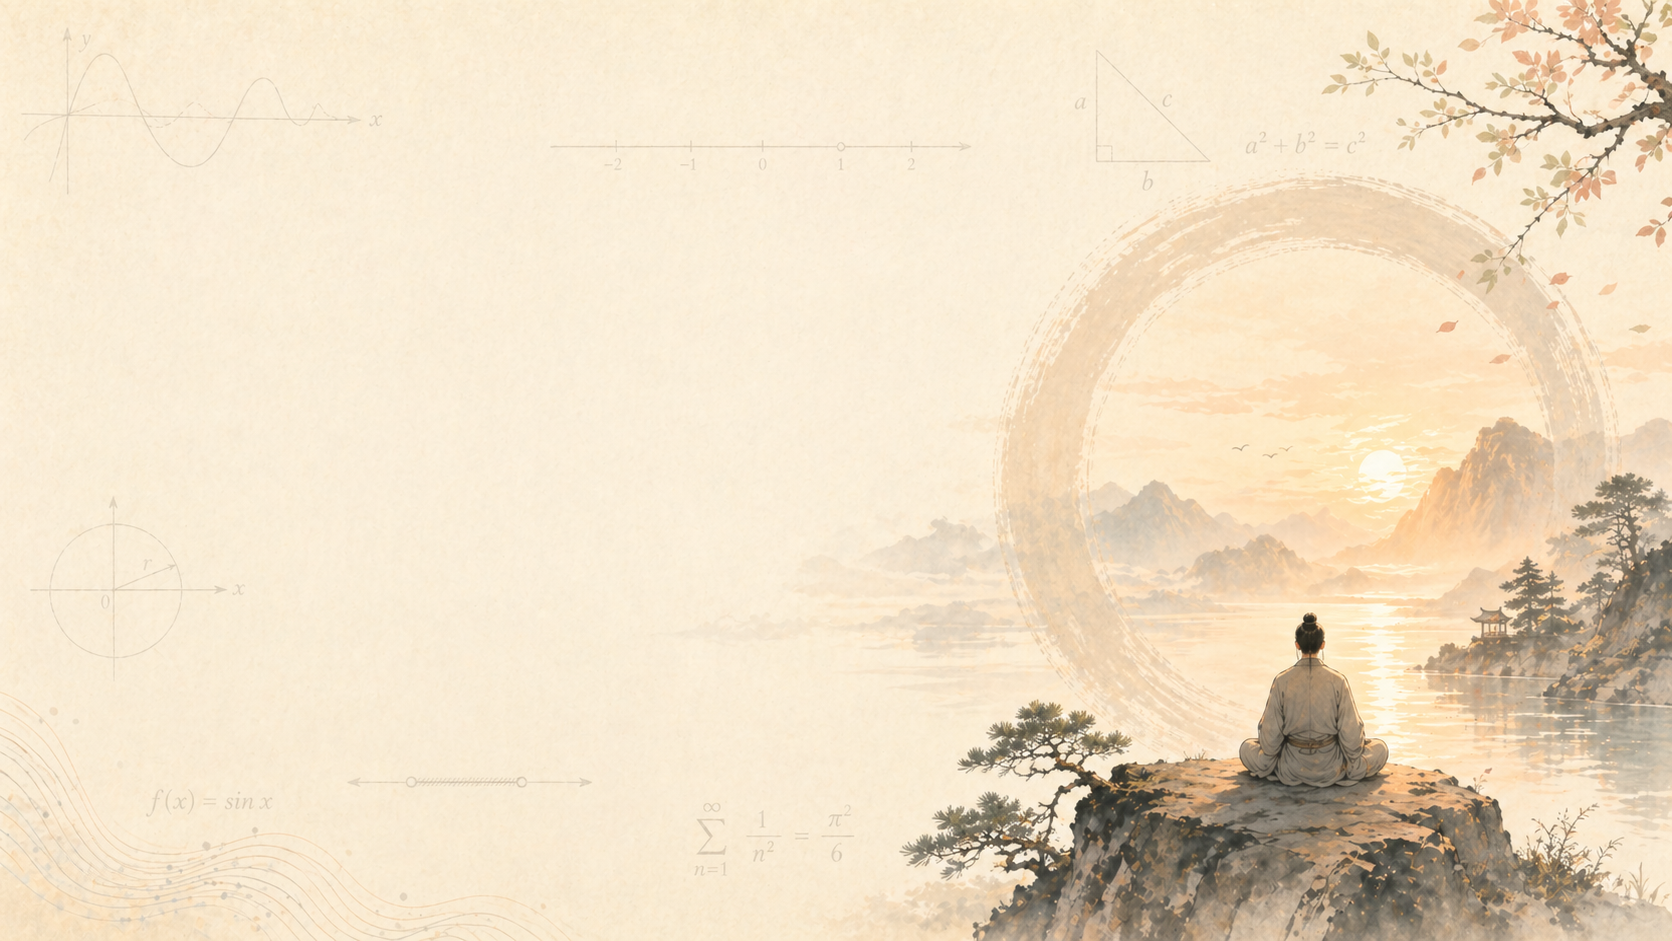
\includegraphics[width=\paperwidth,height=\paperheight,keepaspectratio=false]{chapter_03_bg_01.png}%
}
\begin{frame}[c]{Outline}
  \begin{center}
    \tableofcontents
  \end{center}
  \note{
    Here is the plan. After motivation, we give Definition 3.15,
    which formalises divergence to plus and minus infinity. Then
    Definition 3.16 introduces the set of subsequential limits in
    the extended reals, and from it the upper limit "s" star and
    the lower limit "s" sub star. Theorem 3.17 records the two key
    properties that characterise the upper limit, and we work
    through its proof in cases. Examples 3.18 give us a feel for
    the new objects, including the important fact that the
    ordinary limit exists exactly when the upper and lower limits
    agree. We close with the comparison theorem 3.19.
  }
\end{frame}

% =============================================================================
% MOTIVATION
% =============================================================================
\section{Motivation}

% --- Build 1/4 ---
\begin{frame}{Why Upper and Lower Limits?}
  \begin{hlbox}
    \begin{itemize}
      \item Many sequences \alert{fail to converge} (oscillation, divergence)
    \end{itemize}
  \end{hlbox}

  \note{
    Many real sequences we meet in practice simply fail to
    converge. They may oscillate, like the sequence whose values
    alternate between plus 1 and minus 1, or they may grow without
    bound. The plain notion of limit then has nothing to say about
    them, and we lose a useful summary of their long-run behaviour.
  }
\end{frame}

% --- Build 2/4 ---
\begin{frame}{Why Upper and Lower Limits?}
  \begin{hlbox}
    \begin{itemize}
      \item Many sequences \alert{fail to converge} (oscillation, divergence)
      \item Yet they often have a clear \emph{asymptotic ceiling and floor}
    \end{itemize}
  \end{hlbox}

  \note{
    Even when the limit does not exist, a sequence often has a
    clear upper and lower envelope in the long run. Think of a
    wave whose amplitude settles down to a fixed range. The terms
    keep dancing inside that range without picking out a single
    limit value, but the range itself is unambiguous, and we want
    a way to talk about it.
  }
\end{frame}

% --- Build 3/4 ---
\begin{frame}{Why Upper and Lower Limits?}
  \begin{hlbox}
    \begin{itemize}
      \item Many sequences \alert{fail to converge} (oscillation, divergence)
      \item Yet they often have a clear \emph{asymptotic ceiling and floor}
      \item \alert{Idea:} take \emph{sup} and \emph{inf} of all subsequential limits
    \end{itemize}
  \end{hlbox}

  \note{
    The subsequences of a sequence often do converge, even when
    the sequence as a whole does not, and their limits give us a
    finer record of what is going on. Recall from Section 2 that a
    number is a subsequential limit if some subsequence converges
    to it. We collect all such values, together with possibly plus
    and minus infinity, into a single set, and we will define our
    two new quantities as the supremum and infimum of that set.
  }
\end{frame}

% --- Build 4/4 ---
\begin{frame}{Why Upper and Lower Limits?}
  \begin{hlbox}
    \begin{itemize}
      \item Many sequences \alert{fail to converge} (oscillation, divergence)
      \item Yet they often have a clear \emph{asymptotic ceiling and floor}
      \item \alert{Idea:} take \emph{sup} and \emph{inf} of all subsequential limits
      \item Result: $\limsup$ and $\liminf$ \alert{always exist} in $[-\infty, +\infty]$
    \end{itemize}
  \end{hlbox}

  \note{
    The payoff is that the upper limit and the lower limit always
    exist, in the extended real number system, no matter how badly
    behaved the sequence is. They give us a uniform language for
    asymptotic behaviour, and they reduce to the ordinary limit
    exactly when the sequence does converge. Let us begin with the
    divergent case, where we extend the arrow notation.
  }
\end{frame}

}

{
\usebackgroundtemplate{%
  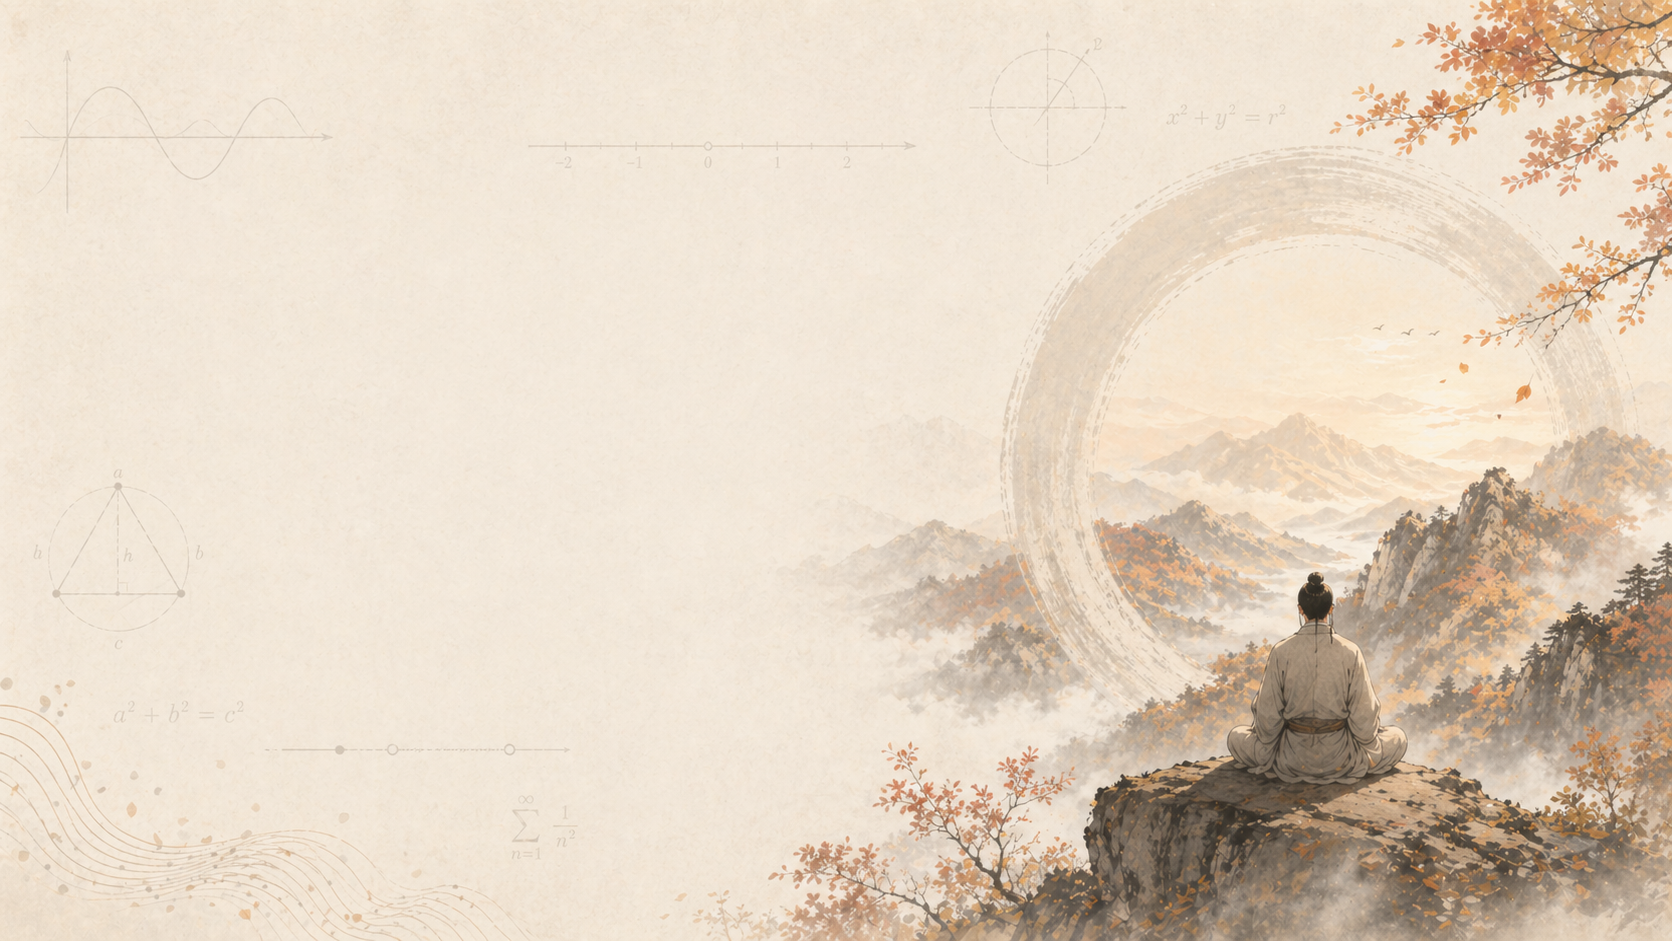
\includegraphics[width=\paperwidth,height=\paperheight,keepaspectratio=false]{chapter_03_bg_02.png}%
}
% =============================================================================
% DEFINITION 3.15: DIVERGENCE TO INFINITY
% =============================================================================
\section{Divergence to Infinity}

% --- Definition 3.15 ---
\begin{frame}{Definition 3.15: Divergence to $\pm\infty$}
  \begin{defblock}{Definition 3.15 --- Divergence to $\pm\infty$}
    Let $\{s_n\}$ be a sequence of real numbers.
    \begin{itemize}
      \item $s_n \to +\infty$ if $\;\forall\, M \in \mathbb{R},\; \exists\, N$ with
        \[
          n \geq N \;\Longrightarrow\; s_n \geq M.
        \]
      \item $s_n \to -\infty$ if $\;\forall\, M \in \mathbb{R},\; \exists\, N$ with
        \[
          n \geq N \;\Longrightarrow\; s_n \leq M.
        \]
    \end{itemize}
  \end{defblock}

  \note{
    The definition formalises what it means for a sequence to grow
    without bound. The first version says: no matter how high a
    target value "M" we pick, the sequence eventually stays at or
    above "M" for the rest of time. The second version is
    symmetric: no matter how low a target "M" we pick, the
    sequence eventually stays at or below it. The role of "M" is
    the same as the role of epsilon in ordinary convergence; it
    lets us quantify how far out we have to go.
  }
\end{frame}

% --- Picture: divergence to +infty ---
\begin{frame}{Picture: $s_n \to +\infty$}
  \begin{center}
  \begin{tikzpicture}[scale=0.8]
    % Axes
    \draw[->, thick, mDarkTeal] (0,0) -- (10.5,0) node[right]{$n$};
    \draw[->, thick, mDarkTeal] (0,-0.3) -- (0,5.2) node[above]{$s_n$};
    % Threshold M
    \draw[dashed, mAccent, thick] (0, 3) -- (10, 3) node[right]{$M$};
    % Vertical line at N
    \draw[dashed, mAccent, thick] (5, 0) -- (5, 5) node[above]{$N$};
    % Sequence dots, increasing then above M
    \fill[defcolor] (0.6, 0.4) circle (2.5pt);
    \fill[defcolor] (1.2, 1.0) circle (2.5pt);
    \fill[defcolor] (1.8, 0.7) circle (2.5pt);
    \fill[defcolor] (2.4, 1.6) circle (2.5pt);
    \fill[defcolor] (3.0, 1.3) circle (2.5pt);
    \fill[defcolor] (3.6, 2.1) circle (2.5pt);
    \fill[defcolor] (4.2, 2.6) circle (2.5pt);
    \fill[defcolor] (4.8, 2.9) circle (2.5pt);
    \fill[thmcolor] (5.4, 3.2) circle (2.5pt);
    \fill[thmcolor] (6.0, 3.5) circle (2.5pt);
    \fill[thmcolor] (6.6, 3.7) circle (2.5pt);
    \fill[thmcolor] (7.2, 3.9) circle (2.5pt);
    \fill[thmcolor] (7.8, 4.2) circle (2.5pt);
    \fill[thmcolor] (8.4, 4.4) circle (2.5pt);
    \fill[thmcolor] (9.0, 4.6) circle (2.5pt);
  \end{tikzpicture}
  \end{center}

  \vspace{0.4em}
  \begin{center}
    \hl{\emph{Past index $N$, all terms lie at or above the threshold $M$.}}
  \end{center}

  \note{
    Here is the picture for divergence to plus infinity. The
    horizontal axis is the index "n" and the vertical axis is the
    value "s" sub "n". The dashed orange horizontal line at height
    "M" is the threshold we are testing against, and the dashed
    vertical line at "N" marks the cutoff. The blue dots show
    early terms scattered below the threshold; the red dots past
    index "N" all lie at or above "M". The point of the
    definition is that we can repeat this picture for any target
    "M", by choosing "N" large enough.
  }
\end{frame}

% --- Remark on -> notation ---
\begin{frame}{Remark on the Notation $\to$}
  \begin{remblock}{Remark}
    Definition 3.15 reuses the symbol $\to$ for certain \alert{divergent} sequences,
    in addition to convergent ones.

    \vspace{0.3em}
    The definition of convergence and limit (Def. 3.1) is \emph{in no way changed}.
  \end{remblock}

  \note{
    A small but important warning about notation. We are now
    writing arrow plus infinity for sequences that diverge in this
    strong sense, even though strictly speaking they do not
    converge to anything in the ordinary metric-space sense. The
    arrow is the same symbol we used in Definition 3.1, but it is
    being applied to a different situation. The original
    definition of convergence and of limit is in no way changed;
    this is purely a notational extension to cover divergence to
    plus or minus infinity.
  }
\end{frame}

}

{
\usebackgroundtemplate{%
  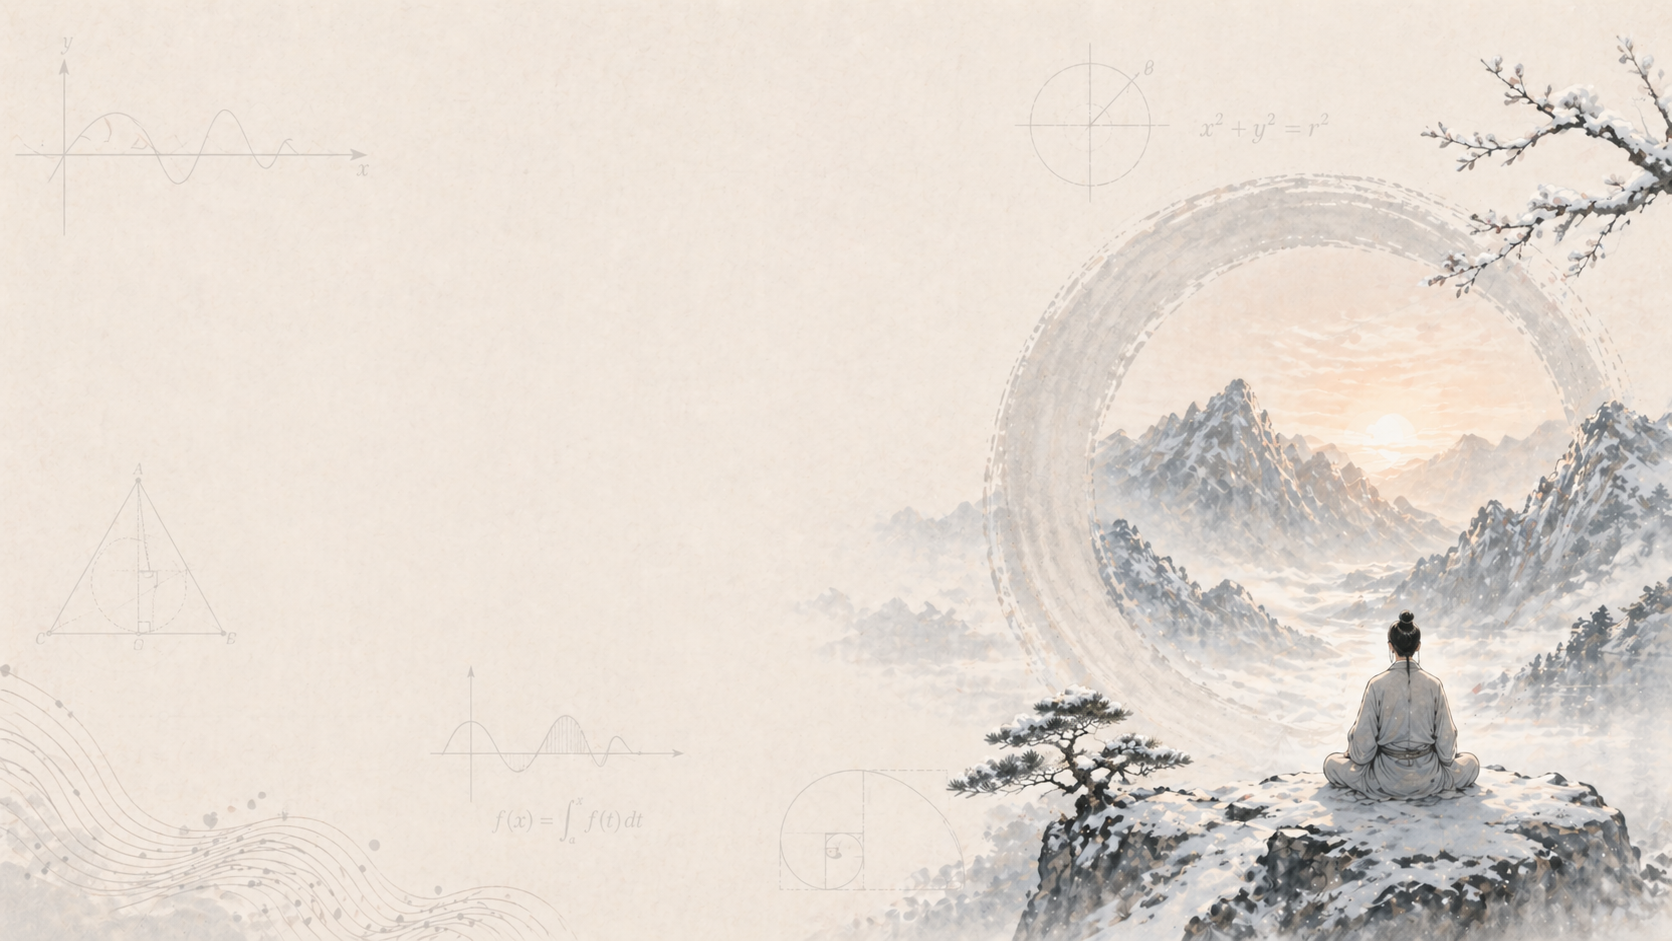
\includegraphics[width=\paperwidth,height=\paperheight,keepaspectratio=false]{chapter_03_bg_03.png}%
}
% =============================================================================
% DEFINITION 3.16: UPPER AND LOWER LIMITS
% =============================================================================
\section{Upper and Lower Limits}

% --- Definition 3.16: Build 1/3 ---
\begin{frame}{Definition 3.16: The Set $E$ of Subsequential Limits}
  \hl{Let $\{s_n\}$ be a real sequence. Define}
  \begin{defblock}{The Set $E$}
    \[
      E = \big\{\, x \in [-\infty, +\infty] \;:\; s_{n_k} \to x \text{ for some subsequence } \{s_{n_k}\}\,\big\}.
    \]
  \end{defblock}

  \vspace{0.4em}
  \begin{hlbox}
    $E$ contains all real subsequential limits (Def. 3.5), \alert{plus possibly} $\pm\infty$.
  \end{hlbox}

  \note{
    The starting point is to collect all the asymptotic values the
    sequence can produce. Look at every subsequence, and record
    what it converges to. The values live in the extended real
    line, so plus infinity and minus infinity are allowed if some
    subsequence diverges to them. The set "E" is the catalogue of
    all these values. It contains the ordinary subsequential
    limits we introduced in Definition 3.5, and possibly the two
    infinities as well.
  }
\end{frame}

% --- Definition 3.16: Build 2/3 ---
\begin{frame}{Definition 3.16: Upper and Lower Limits}
  \begin{defblock}{Definition 3.16 --- Upper and Lower Limits}
    \[
      s^* = \sup E, \qquad s_* = \inf E.
    \]
    The numbers $s^*$ and $s_*$ are the \alert{upper} and \alert{lower limits} of $\{s_n\}$.
  \end{defblock}

  \vspace{0.5em}
  \begin{hlbox}
    Sup and inf are taken in $[-\infty, +\infty]$ (Definitions 1.8 and 1.23).
  \end{hlbox}

  \note{
    Now we extract two single numbers from the set "E". The
    supremum of "E", taken in the extended real line, is the upper
    limit "s" star. The infimum of "E" is the lower limit "s" sub
    star. Because supremum and infimum are taken in the extended
    line, they always exist; the worst that can happen is that
    they are plus or minus infinity. So upper and lower limits
    are universal: every real sequence has them.
  }
\end{frame}

% --- Definition 3.16: Build 3/3 ---
\begin{frame}{Definition 3.16: Notation $\limsup$ and $\liminf$}
  \begin{defblock}{Definition 3.16 --- Notation}
    \[
      \limsup_{n \to \infty} s_n = s^*, \qquad \liminf_{n \to \infty} s_n = s_*.
    \]
  \end{defblock}

  \vspace{0.5em}
  \begin{hlbox}
    \textbf{Read as:} the \emph{limit superior} (or \emph{upper limit}) and
    the \emph{limit inferior} (or \emph{lower limit}) of $\{s_n\}$.
  \end{hlbox}

  \note{
    Two pieces of standard notation. The upper limit is written
    "lim sup" of "s" sub "n" as "n" goes to infinity, and the
    lower limit is written "lim inf". You will also hear them
    called the limit superior and limit inferior. The names are
    well chosen: each is a kind of limit, in a generalised sense,
    that always exists, even when the ordinary limit does not.
    Whenever the ordinary limit does exist, both will collapse
    onto it, as we will see in a moment. We will use these
    symbols frequently from here on, especially in the
    convergence tests for series later in this chapter, where
    the ordinary limit is often unavailable but the limsup is
    always at hand. With the notation in place, let us draw a
    picture.
  }
\end{frame}

% --- Picture: E with limsup and liminf ---
\begin{frame}{Picture: $E$, $\limsup$, and $\liminf$}
  \begin{center}
  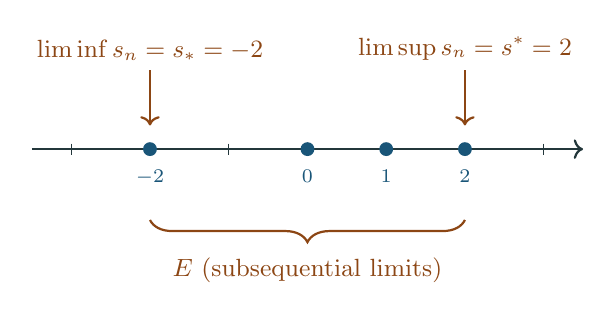
\begin{tikzpicture}[xscale=1.0, yscale=1.0]
    % Number line with integer ticks; dots placed at their actual values
    \draw[->, thick, mDarkTeal] (-3.5,0) -- (3.5,0);
    % Tick marks at integer positions
    \foreach \x in {-3,-2,-1,0,1,2,3} {
      \draw[mDarkTeal] (\x, 0.07) -- (\x, -0.07);
    }
    % Subsequential limits at their actual values
    \fill[defcolor] (-2, 0) circle (2.5pt) node[below=4pt]{\scriptsize $-2$};
    \fill[defcolor] ( 0, 0) circle (2.5pt) node[below=4pt]{\scriptsize $0$};
    \fill[defcolor] ( 1, 0) circle (2.5pt) node[below=4pt]{\scriptsize $1$};
    \fill[defcolor] ( 2, 0) circle (2.5pt) node[below=4pt]{\scriptsize $2$};
    % Brace under E
    \draw[thick, mAccent, decorate, decoration={brace, amplitude=8pt, mirror}]
      (-2, -0.9) -- (2, -0.9) node[midway, below=10pt]{\small $E$ (subsequential limits)};
    % Inf and sup labels above
    \draw[<-, thick, mAccent] (-2, 0.3) -- (-2, 1.0) node[above]{\small $\liminf s_n = s_* = -2$};
    \draw[<-, thick, mAccent] ( 2, 0.3) -- ( 2, 1.0) node[above]{\small $\limsup s_n = s^* = 2$};
  \end{tikzpicture}
  \end{center}

  \vspace{0.5em}
  \begin{center}
    \hl{\emph{$\liminf$ is the smallest, $\limsup$ the largest subsequential limit.}}
  \end{center}

  \note{
    Here is the geometric picture. The horizontal axis is the
    extended real line. The four blue dots mark the subsequential
    limits of some imaginary sequence: minus 2, 0, 1, and 2. The
    orange brace below shows the entire set "E" of these values.
    The upper limit is the largest, sitting at 2, and the lower
    limit is the smallest, sitting at minus 2. In general the set
    "E" can be much bigger than four points; it can be a whole
    interval, or even the entire extended line. But the upper and
    lower limits are always its supremum and infimum.
  }
\end{frame}

% --- Observation: E is non-empty ---
\begin{frame}{Observation: $E$ Is Always Non-Empty}
  \begin{remblock}{Observation}
    For every real sequence $\{s_n\}$, the set $E$ is \alert{non-empty}: \\
    so $\limsup s_n$ and $\liminf s_n$ are always well-defined.
  \end{remblock}

  \vspace{0.3em}
  \begin{proofblock}{Three cases}
    \begin{enumerate}
      \item[(1)] $\{s_n\}$ \emph{unbounded above} $\;\Longrightarrow\;$ some $s_{n_k} \to +\infty$. \quad So $+\infty \in E$.
      \item[(2)] $\{s_n\}$ \emph{unbounded below} $\;\Longrightarrow\;$ some $s_{n_k} \to -\infty$. \quad So $-\infty \in E$.
      \item[(3)] $\{s_n\}$ \emph{bounded in $\mathbb{R}$:} all terms lie in a compact interval $[L, U]$.
        By Bolzano-Weierstrass Theorem 3.6, there exists a subsequence $s_{n_k} \to p \in [L, U]$. So $p \in E$. \quad $\Box$
    \end{enumerate}
  \end{proofblock}

  \note{
    Before going further, an important observation: the set "E"
    is never empty. Some asymptotic value always exists, so the
    upper and lower limits are always well-defined. The argument
    splits into three cases. First, if the sequence is not
    bounded above, we can pick out terms growing arbitrarily
    large, giving a subsequence diverging to plus infinity, so
    plus infinity belongs to "E". Second, by symmetry, if the
    sequence is not bounded below, some subsequence diverges to
    minus infinity, so minus infinity belongs to "E". Third, if
    the sequence is bounded in the reals, then all its terms lie
    in some closed bounded, hence compact, interval. By Theorem
    3.6, the Bolzano-Weierstrass theorem from Section 2, some
    subsequence converges to a point "p" in that interval, and
    "p" belongs to "E". In every case "E" contains at least one
    point, so it is non-empty.
  }
\end{frame}

}

{
\usebackgroundtemplate{%
  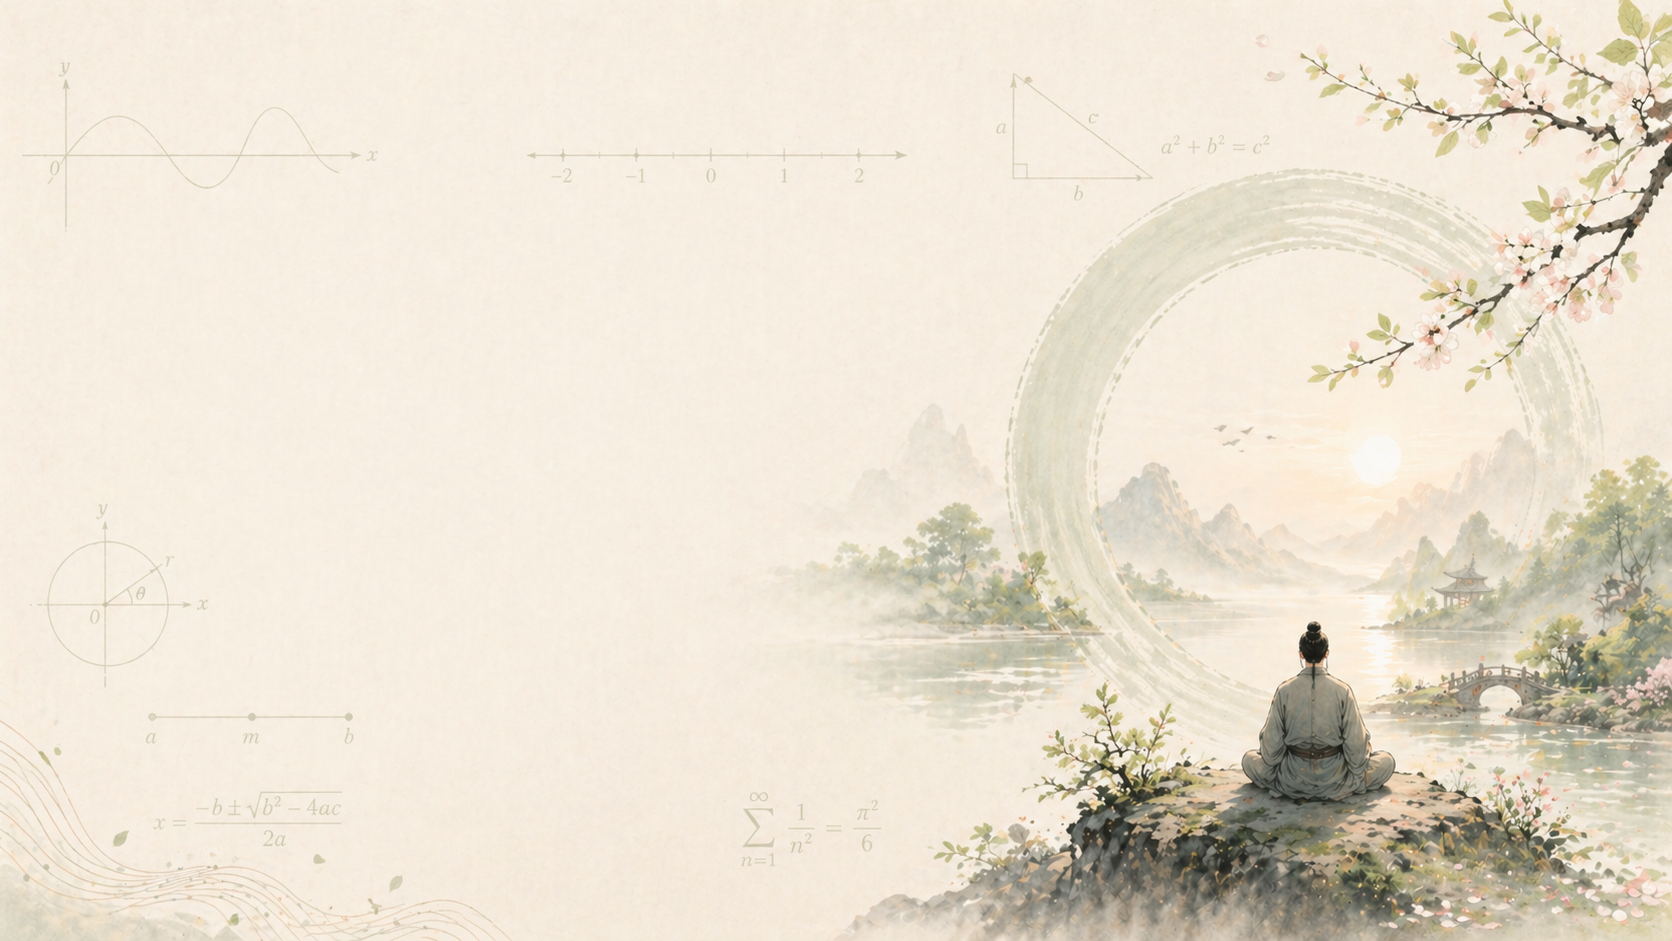
\includegraphics[width=\paperwidth,height=\paperheight,keepaspectratio=false]{chapter_03_bg_04.png}%
}
% =============================================================================
% THEOREM 3.17: PROPERTIES OF s*
% =============================================================================
\section{Properties of the Upper Limit}

% --- Theorem 3.17: Build 1/3 ---
\begin{frame}{Theorem 3.17: Two Properties of $s^*$}
  \hl{Let $\{s_n\}$ be a real sequence; $E$ and $s^*$ as in Definition 3.16.}
  \begin{thmblock}{Theorem 3.17}
    \begin{itemize}
      \item[(a)] $s^* \in E$.
    \end{itemize}
  \end{thmblock}

  \note{
    Theorem 3.17 pins down the upper limit by listing two
    properties that determine it uniquely. The first property says
    that "s" star is itself a subsequential limit, that is, "s"
    star belongs to the set "E". The supremum of "E" is achieved
    as one of its members. This is not automatic for general sets;
    it relies on the specific structure of "E".
  }
\end{frame}

% --- Theorem 3.17: Build 2/3 ---
\begin{frame}{Theorem 3.17: Two Properties of $s^*$}
  \hl{Let $\{s_n\}$ be a real sequence; $E$ and $s^*$ as in Definition 3.16.}
  \begin{thmblock}{Theorem 3.17}
    \begin{itemize}
      \item[(a)] $s^* \in E$.
      \item[(b)] If $x > s^*$, there is $N$ such that $n \geq N$ implies $s_n < x$.
    \end{itemize}
  \end{thmblock}

  \note{
    The second property says that nothing strictly above "s" star
    can be reached infinitely often. Pick any threshold "x"
    larger than "s" star; then the sequence eventually stays
    below "x". So while "s" star is achieved as a subsequential
    limit, nothing above it is. This is the upper-bound aspect of
    the supremum, expressed in sequence language.
  }
\end{frame}

% --- Theorem 3.17: Build 3/3 ---
\begin{frame}{Theorem 3.17: Two Properties of $s^*$}
  \hl{Let $\{s_n\}$ be a real sequence; $E$ and $s^*$ as in Definition 3.16.}
  \begin{thmblock}{Theorem 3.17}
    \begin{itemize}
      \item[(a)] $s^* \in E$.
      \item[(b)] If $x > s^*$, there is $N$ such that $n \geq N$ implies $s_n < x$.
    \end{itemize}

    \vspace{0.3em}
    Moreover, $s^*$ is the \alert{only} number with properties (a) and (b).
  \end{thmblock}

  \hl{An analogous statement holds for $s_*$.}

  \note{
    Together properties "a" and "b" pin down a single number. The
    theorem asserts that "s" star is the only candidate satisfying
    both. So we have an alternative description of the upper
    limit, sometimes more useful in proofs: it is the unique value
    that is itself a subsequential limit, and above which the
    sequence eventually does not return. The same statement, with
    inequalities reversed, characterises the lower limit "s" sub
    star.
  }
\end{frame}

% --- Picture: properties of s* ---
\begin{frame}{Picture: The Two Properties of $s^*$}
  \begin{center}
  \begin{tikzpicture}[scale=1.0]
    % Number line
    \draw[->, thick, mDarkTeal] (-5.5,0) -- (5.5,0);
    % Subsequential limits and s*
    \fill[defcolor] (-3.5, 0) circle (2pt);
    \fill[defcolor] (-1.5, 0) circle (2pt);
    \fill[defcolor] (0.0, 0) circle (2pt);
    \fill[thmcolor] (1.5, 0) circle (3.5pt) node[below=6pt, thmcolor]{$s^*$};
    % x > s*
    \draw[dashed, mAccent, thick] (3.0, -0.4) -- (3.0, 1.4);
    \node[mAccent, above=2pt] at (3.0, 1.4) {\small $x > s^*$};
    % Arrow indicating tail < x
    \draw[<-, thick, mAccent] (3.0, 0.7) -- (4.7, 0.7);
    \node[mAccent, right=0pt] at (4.7, 0.7) {\small $s_n < x$ eventually};
    % Brace under E
    \draw[thick, defcolor, decorate, decoration={brace, amplitude=6pt, mirror}]
      (-3.5, -0.9) -- (1.5, -0.9) node[midway, below=8pt, defcolor]{\small $E$};
  \end{tikzpicture}
  \end{center}

  \vspace{0.4em}
  \begin{center}
    \begin{hlbox}
      \textbf{(a)} $s^*$ is reached by some subsequence. \\
      \textbf{(b)} Nothing above $s^*$ is reached infinitely often.
    \end{hlbox}
  \end{center}

  \note{
    Here is the picture in cartoon form. The horizontal axis is
    the real line. The orange brace below spans the entire set
    "E" of subsequential limits; the smaller blue dots are some
    of the values in "E", and the larger red dot at the right
    end of the brace is "s" star, the largest value in "E".
    Property "a" is the statement that the red dot belongs to
    "E"; that is, some subsequence actually converges to "s"
    star. Property "b" looks to the right of "s" star: pick any
    threshold "x" strictly above the red dot, drawn as the
    dashed orange vertical line, and the sequence eventually
    stays to the left of it, with no return trips. So nothing
    from "E" can sit to the right of "s" star. Both properties
    are visible in this single picture.
  }
\end{frame}

% --- Proof Strategy ---
\begin{frame}{Proof Strategy: Theorem 3.17}
  \begin{hlbox}
    \textbf{Goal:} (a) $s^* \in E$; \;(b) $s_n < x$ eventually for $x > s^*$; \;and uniqueness.

    \vspace{0.6em}
    \textbf{Plan for (a):} \emph{three cases} on the value of $s^*$.
    \begin{itemize}
      \item $s^* = +\infty$: $\{s_n\}$ unbounded above $\;\Longrightarrow\;$ subsequence $\to +\infty$.
      \item $s^*$ real: invoke Theorems 3.7 and 2.28.
      \item $s^* = -\infty$: only $-\infty$ in $E$; $s_n \to -\infty$.
    \end{itemize}

    \vspace{0.6em}
    \textbf{Plan for (b):} $s_n \geq x$ infinitely often forces a $y \in E$ with $y \geq x > s^*$, which contradicts $s^* = \sup E$.

    \vspace{0.4em}
    \textbf{Uniqueness:} if $p < q$ both work, an $x \in (p,q)$ contradicts (a) at $q$.
  \end{hlbox}

  \note{
    Before diving in, here is the high-level strategy. For
    property "a" we split into three cases according to whether
    the upper limit is plus infinity, a real number, or minus
    infinity, and we handle each separately. For property "b" we
    argue by contradiction: assuming the conclusion fails produces
    a subsequential limit above "s" star, which is impossible.
    Uniqueness follows from one short observation. Let us go
    through each case in turn.
  }
\end{frame}

% --- Proof of (a): case s* = +infty ---
\begin{frame}{Proof of (a): $s^* \in E$ \quad [Case $s^* = +\infty$]}
  \begin{proofblock}{$s^* = +\infty$}
    $s^* = \sup E = +\infty$ implies that $\{s_n\}$ is unbounded above. \\
    (If $\{s_n\}$ was bounded above, $E$ would also be bounded above.) \\
    Thus there exists a subsequence $\{s_{n_k}\}$ such that $s_{n_k} \to +\infty$.

    \vspace{0.3em}
    Therefore $+\infty \in E$, that is, $s^* \in E$.
  \end{proofblock}

  \note{
    Start with the case that "s" star equals plus infinity. By
    definition, this means "E" has no real upper bound, so "E" is
    unbounded above as a set. If "E" were unbounded above but the
    sequence "s" sub "n" were bounded above, every subsequence
    would also be bounded, and no subsequential limit could exceed
    that bound. So the sequence itself must be unbounded above.
    From an unbounded sequence we can pick out terms growing
    without bound, giving a subsequence diverging to plus
    infinity. That subsequential limit is plus infinity, which is
    exactly "s" star.
  }
\end{frame}

% --- Proof of (a): case s* real ---
\begin{frame}{Proof of (a): $s^* \in E$ \quad [Case $s^*$ Real]}
  \begin{proofblock}{$s^*$ real}
    $E$ is bounded above and at least one real subsequential limit exists.

    \vspace{0.3em}
    \begin{itemize}
      \item Theorem 3.7: real subsequential limits form a closed subset of $\mathbb{R}$.
      \item Theorem 2.28: $\sup$ of a closed, bounded-above subset of $\mathbb{R}$ lies in that subset.
    \end{itemize}

    \vspace{0.3em}
    Hence $s^* = \sup E \in E$.
  \end{proofblock}

  \note{
    Next, the case where "s" star is a finite real number. Then
    "E" is bounded above. Theorem 3.7 from Section 2 told us that
    the set of subsequential limits is closed; combined with
    boundedness, the set is closed and bounded. Theorem 2.28 from
    Chapter 2 says that the supremum of a closed bounded set of
    real numbers actually belongs to the set. Putting the two
    together, "s" star is in "E".
  }
\end{frame}

% --- Proof of (a): case s* = -infty ---
\begin{frame}{Proof of (a): $s^* \in E$ \quad [Case $s^* = -\infty$]}
  \begin{proofblock}{$s^* = -\infty$}
    $\sup E = -\infty$ forces $E = \{-\infty\}$. \\
    Hence $+\infty \notin E$, so $\{s_n\}$ is bounded above; and no \emph{real} subsequential limit exists.

    \vspace{0.3em}
    Fix any real $M$. If $s_n > M$ for infinitely many $n$, then that subsequence is bounded (both above by the bound on $\{s_n\}$, and below by $M$), so by Bolzano-Weierstrass (Theorem 3.6) it has a real subsequential limit $y \geq M$, \alert{contradicting} $E = \{-\infty\}$.

    \vspace{0.3em}
    Thus $s_n \leq M$ eventually, that is, $s_n \to -\infty$. Hence $s^* = -\infty \in E$. \quad $\Box$
  \end{proofblock}

  \note{
    The last case is "s" star equals minus infinity. The
    supremum of "E" is minus infinity only if "E" itself
    contains nothing above minus infinity, which means "E" is
    just the singleton minus infinity. In particular, plus
    infinity is not in "E", so the sequence is bounded above;
    and no real number is a subsequential limit. Now suppose,
    for some real "M", that "s" sub "n" exceeds "M" for
    infinitely many indices. The corresponding subsequence is
    bounded above by the bound on the original sequence and
    below by "M", so Bolzano-Weierstrass produces a real
    subsequential limit at least "M". That contradicts our
    finding that no real subsequential limit exists. So past
    some index every term lies at or below "M", which is
    exactly divergence to minus infinity. The single element of
    "E" is then minus infinity, equal to "s" star, and we are
    done with part "a".
  }
\end{frame}

% --- Proof of (b) ---
\begin{frame}{Proof of (b): $s_n < x$ eventually for $x > s^*$}
  \begin{proofblock}{If $x > s^*$, then $s_n < x$ eventually}
    Suppose, for contradiction, $s_n \geq x$ for infinitely many $n$. Restrict to that subsequence; all its terms are $\geq x$.

    \vspace{0.3em}
    \begin{itemize}
      \item If \emph{bounded above:} Bolzano-Weierstrass (Theorem 3.6) gives a sub-subsequence with real limit $y \geq x$.
      \item If \emph{unbounded above:} a sub-subsequence diverges to $y = +\infty \geq x$.
    \end{itemize}

    \vspace{0.3em}
    Either way, $y \in E$ with $y \geq x > s^* = \sup E$, \alert{contradiction}. \quad $\Box$
  \end{proofblock}

  \note{
    Now property "b". Argue by contradiction. Suppose the
    conclusion fails: there is some "x" greater than "s" star,
    and yet "s" sub "n" is at least "x" for infinitely many
    indices. Pull out a subsequence consisting of those indices;
    every term is at least "x". Now consider two cases. If this
    subsequence is bounded above, Bolzano-Weierstrass gives a
    sub-subsequence converging to a real "y" at least "x". If
    it is unbounded above, a sub-subsequence diverges to plus
    infinity, which we treat as "y" equals plus infinity, again
    at least "x". In either case "y" is a subsequential limit
    of the original sequence, so "y" belongs to "E". But "y" is
    at least "x", which is strictly greater than the supremum
    of "E". That is impossible, so the contradiction proves "b".
  }
\end{frame}

% --- Proof of uniqueness ---
\begin{frame}{Proof of Uniqueness}
  \begin{proofblock}{Only $s^*$ satisfies (a) and (b)}
    Suppose $p$ and $q$ both satisfy (a) and (b), with $p < q$.

    \vspace{0.3em}
    Choose $x$ with $p < x < q$.

    \vspace{0.3em}
    $p$ satisfies (b): $s_n < x$ for all $n \geq N$.

    \vspace{0.3em}
    $q$ satisfies (a): some subsequence converges to $q > x$. \alert{Impossible.} \quad $\Box$
  \end{proofblock}

  \note{
    For uniqueness, suppose two numbers "p" and "q" both satisfy
    properties "a" and "b", and assume without loss of generality
    that "p" is less than "q". Pick any "x" strictly between
    them. Since "p" satisfies "b", the sequence is eventually
    below "x". But "q" satisfies "a", which means some
    subsequence converges to "q", and "q" is strictly above "x".
    A sequence that is eventually below "x" cannot have a
    subsequential limit above "x". So the two are incompatible,
    and we conclude that there is at most one number with both
    properties. Combined with the existence proof, that unique
    number is "s" star.
  }
\end{frame}

}

{
\usebackgroundtemplate{%
  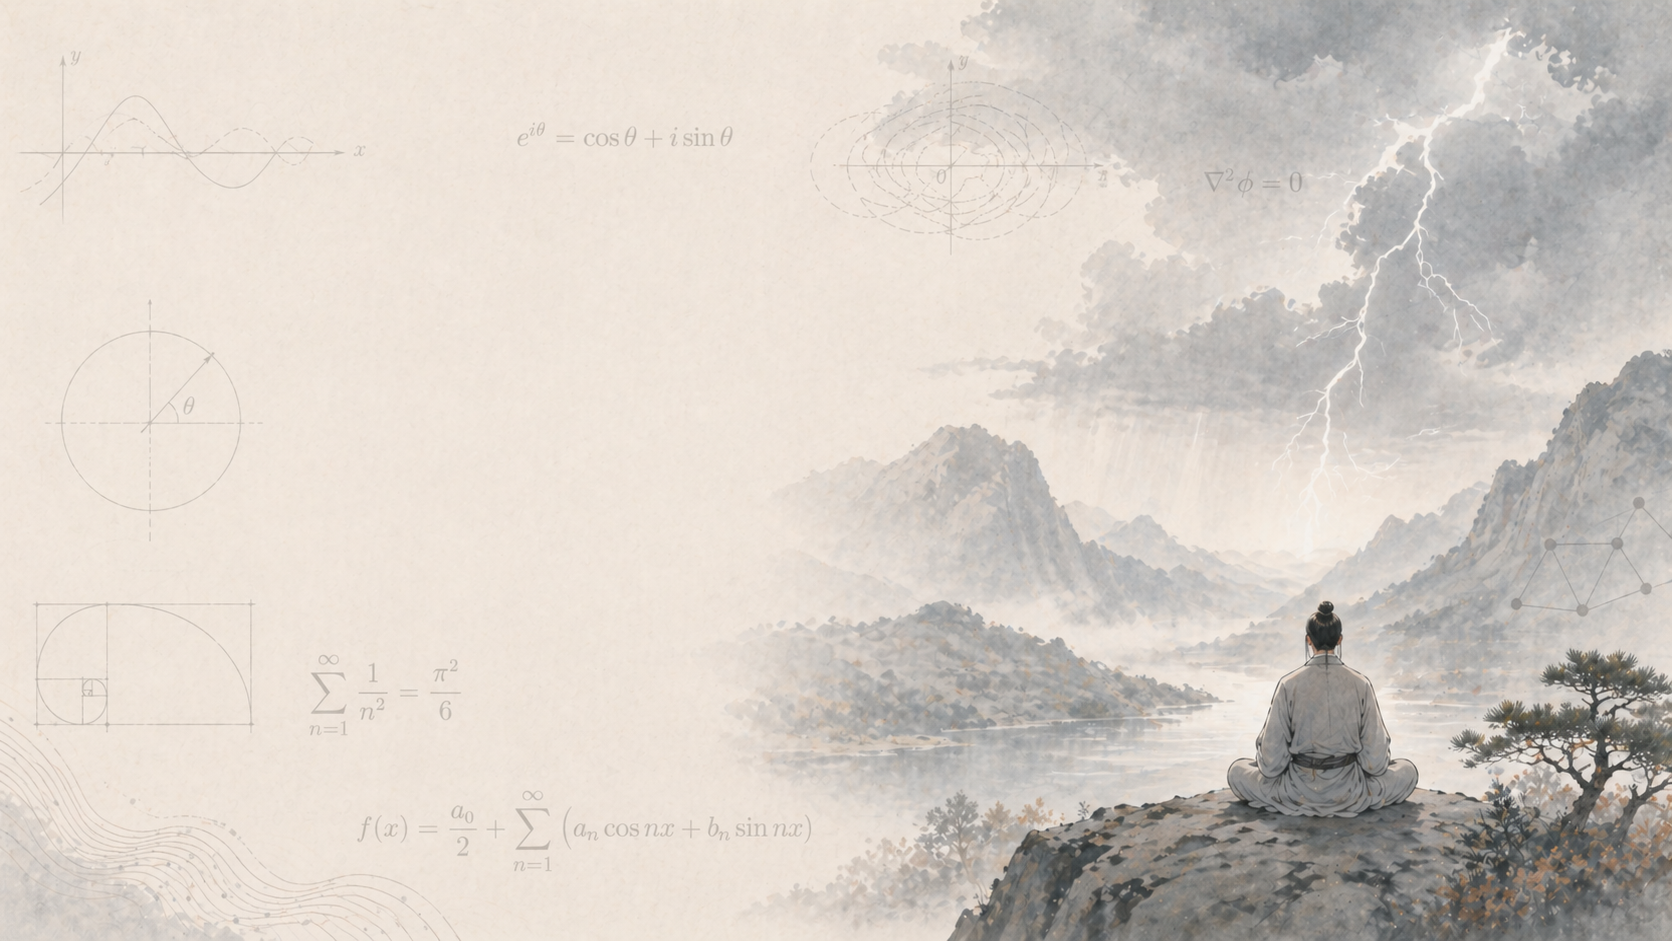
\includegraphics[width=\paperwidth,height=\paperheight,keepaspectratio=false]{chapter_03_bg_05.png}%
}
% =============================================================================
% EXAMPLES 3.18
% =============================================================================
\section{Examples}

% --- Example 3.18 (a) ---
\begin{frame}{Example 3.18 (a): A Sequence Hitting Every Rational}
  \begin{exblock}{Example 3.18 (a)}
    Let $\{s_n\}$ enumerate \alert{all rational numbers}.

    \vspace{0.3em}
    Every real number is a subsequential limit, so $E = [-\infty, +\infty]$.
    \[
      \limsup_{n \to \infty} s_n = +\infty, \qquad \liminf_{n \to \infty} s_n = -\infty.
    \]
  \end{exblock}

  \note{
    The first example is the most extreme. Take any sequence
    whose terms run through all the rational numbers, in some
    order. Such a sequence exists because the rationals are
    countable. Now any real number "x", rational or irrational,
    is the limit of some sequence of rationals, so we can extract
    a subsequence of our sequence converging to "x". In other
    words, every real number is a subsequential limit. Plus and
    minus infinity are also subsequential limits, since the
    rationals contain arbitrarily large positive and negative
    values. So "E" is the entire extended real line, and its
    supremum and infimum are plus and minus infinity.
  }
\end{frame}

% --- Example 3.18 (b) ---
\begin{frame}{Example 3.18 (b): An Oscillating Sequence}
  \begin{exblock}{Example 3.18 (b)}
    Let
    \[
      s_n = \frac{(-1)^n}{1 + 1/n}.
    \]
    Then
    \[
      \limsup_{n \to \infty} s_n = 1, \qquad \liminf_{n \to \infty} s_n = -1.
    \]
  \end{exblock}

  \vspace{0.3em}
  \begin{hlbox}
    \textbf{Why:} the even-$n$ subsequence $\to +1$; the odd-$n$ subsequence $\to -1$.
  \end{hlbox}

  \note{
    The second example is the running prototype. The sequence
    alternates sign by way of minus 1 to the "n" power, and
    multiplies by a factor that approaches 1 as "n" grows. The
    even-indexed terms are positive and converge to plus 1; the
    odd-indexed terms are negative and converge to minus 1. So
    plus 1 and minus 1 are the two subsequential limits, and
    they are also the supremum and infimum of "E". The upper
    limit is 1, and the lower limit is minus 1, even though the
    sequence itself does not converge.
  }
\end{frame}

% --- Picture: example 3.18(b) ---
\begin{frame}{Picture: Example 3.18 (b)}
  \begin{center}
  \begin{tikzpicture}[scale=2.0]
    % Axes (visual x = n/2, so n=10 corresponds to x=5)
    \draw[->, thick, mDarkTeal] (0,0) -- (5.6,0) node[right]{$n$};
    \draw[->, thick, mDarkTeal] (0,-1.2) -- (0,1.3) node[above]{$s_n$};
    % Reference lines at +1 and -1
    \draw[dashed, thmcolor, thick] (0, 1) -- (5.6, 1) node[right, thmcolor]{$+1$};
    \draw[dashed, thmcolor, thick] (0,-1) -- (5.6,-1) node[right, thmcolor]{$-1$};
    % Tick marks labeled with the actual n values
    \foreach \n/\xpos in {1/0.5, 2/1.0, 3/1.5, 4/2.0, 5/2.5, 6/3.0, 7/3.5, 8/4.0, 9/4.5, 10/5.0} {
      \draw[mDarkTeal] (\xpos, 0.04) -- (\xpos, -0.04);
    }
    \foreach \n/\xpos in {2/1.0, 4/2.0, 6/3.0, 8/4.0, 10/5.0} {
      \node[mDarkTeal] at (\xpos, -0.18) {\tiny $\n$};
    }
    % Even n (positive, approaching +1) -- visual x = n/2
    \fill[defcolor] (1.0, 0.667) circle (1.5pt);
    \fill[defcolor] (2.0, 0.800) circle (1.5pt);
    \fill[defcolor] (3.0, 0.857) circle (1.5pt);
    \fill[defcolor] (4.0, 0.889) circle (1.5pt);
    \fill[defcolor] (5.0, 0.909) circle (1.5pt);
    % Odd n (negative, approaching -1) -- visual x = n/2
    \fill[excolor] (0.5, -0.500) circle (1.5pt);
    \fill[excolor] (1.5, -0.750) circle (1.5pt);
    \fill[excolor] (2.5, -0.833) circle (1.5pt);
    \fill[excolor] (3.5, -0.875) circle (1.5pt);
    \fill[excolor] (4.5, -0.900) circle (1.5pt);
    % Labels for the two subsequences
    \node[defcolor] at (5.3, 0.45) {\scriptsize even $n$};
    \node[excolor] at (5.3, -0.45) {\scriptsize odd $n$};
  \end{tikzpicture}
  \end{center}

  \vspace{0.3em}
  \begin{center}
    \hl{\emph{Two interlaced subsequences with limits $\pm 1$.}}
  \end{center}

  \note{
    The picture shows the two subsequences side by side. The
    horizontal axis is the index "n" and the vertical axis is the
    value "s" sub "n". The upper dashed red line at height plus 1
    and the lower dashed red line at height minus 1 are the two
    asymptotic levels. The blue dots are the even-indexed terms,
    creeping up toward plus 1 from below; the orange dots are the
    odd-indexed terms, creeping down toward minus 1 from above.
    The original sequence interlaces these two strands and never
    settles, but each strand converges. The upper level is the
    limit superior, and the lower level is the limit inferior.
  }
\end{frame}

% --- Example 3.18 (c) ---
\begin{frame}{Example 3.18 (c): Convergence Criterion}
  \begin{exblock}{Example 3.18 (c)}
    For a real sequence $\{s_n\}$:
    \[
      \lim_{n \to \infty} s_n = s
      \quad \iff \quad
      \limsup_{n \to \infty} s_n = \liminf_{n \to \infty} s_n = s.
    \]
  \end{exblock}

  \vspace{0.4em}
  \begin{remblock}{Why this matters}
    The ordinary limit exists \alert{exactly when} $\limsup$ and $\liminf$ \alert{agree}. \\
    All asymptotic information is captured by the two extremes.
  \end{remblock}

  \note{
    The third example is the most useful general fact: a real
    sequence converges to "s" if and only if both its upper and
    lower limits equal "s". The forward direction is
    straightforward. If the sequence converges to "s", every
    subsequence also converges to "s", so "E" is just the single
    point "s", and its supremum and infimum both equal "s". For
    the converse, suppose limsup equals liminf equals "s". Then
    "E" is just "s" alone. If the original sequence did not
    converge to "s", we could pull out a subsequence whose terms
    all stay away from "s" by some fixed positive distance. By
    compactness of the extended real line, that subsequence
    would have a sub-subsequence converging to some point, and
    that point would be a subsequential limit of the original
    sequence different from "s", contradicting "E" being just
    one point. So the sequence must converge to "s". The
    practical takeaway: limsup and liminf together carry all the
    asymptotic information about the sequence; convergence is
    nothing more than the two of them agreeing.
  }
\end{frame}

}

{
\usebackgroundtemplate{%
  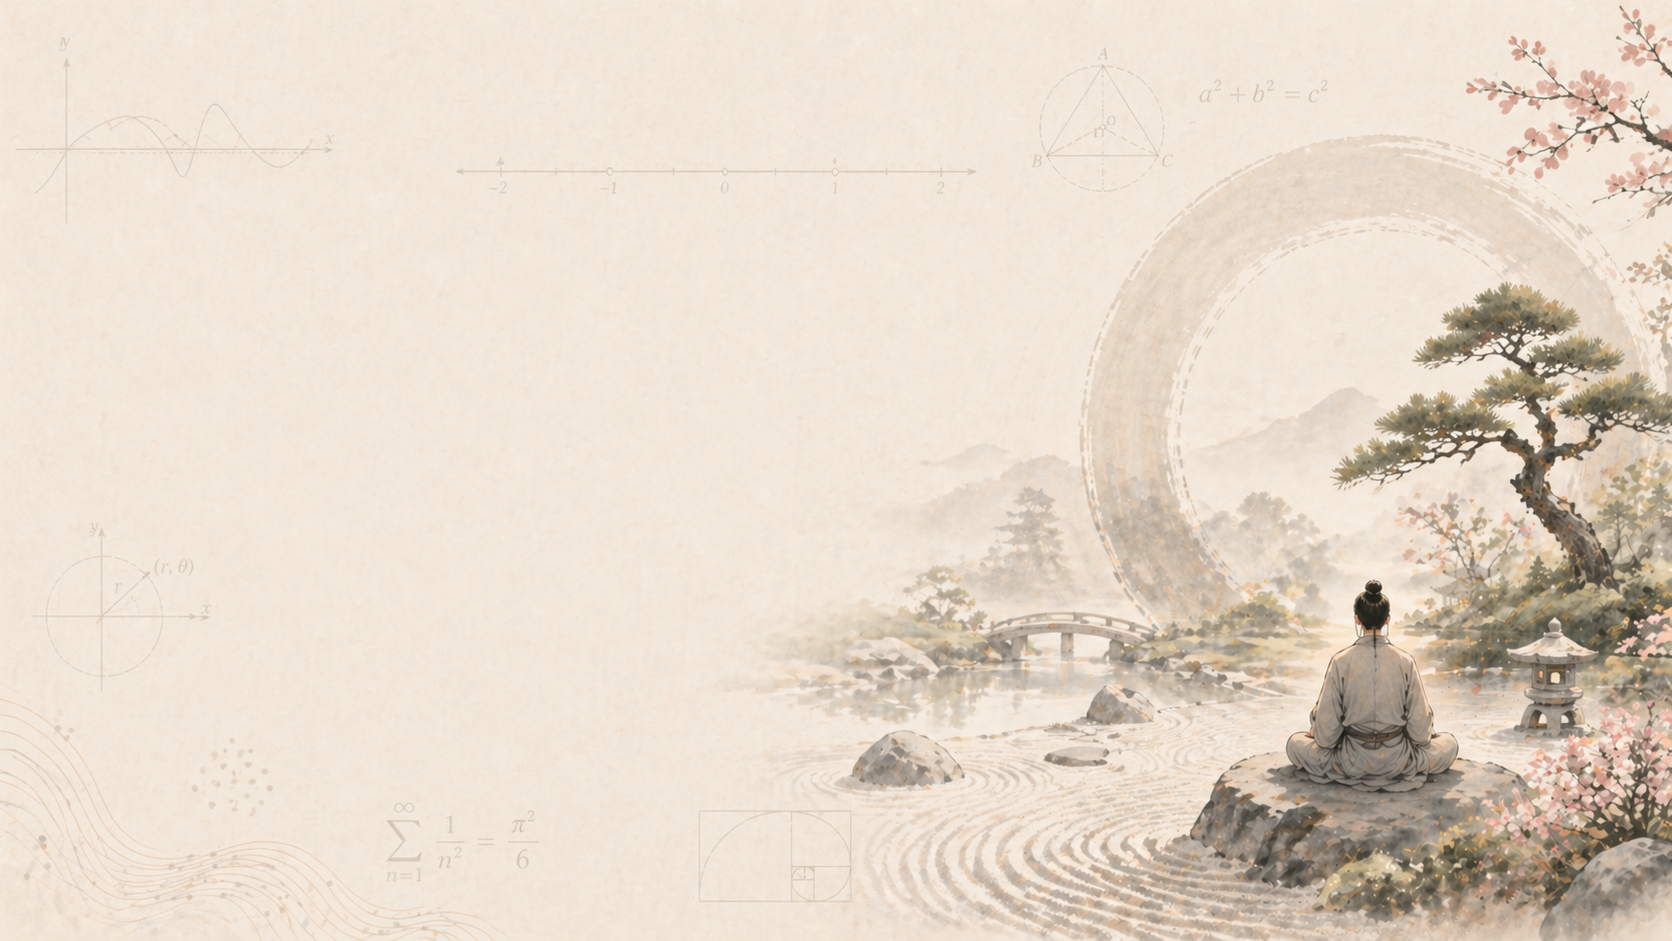
\includegraphics[width=\paperwidth,height=\paperheight,keepaspectratio=false]{chapter_03_bg_06.png}%
}
% =============================================================================
% THEOREM 3.19: COMPARISON
% =============================================================================
\section{Comparing Sequences}

% --- Theorem 3.19 ---
\begin{frame}{Theorem 3.19: Order Is Preserved}
  \begin{thmblock}{Theorem 3.19}
    If $s_n \leq t_n$ for $n \geq N$ (some fixed $N$), then
    \[
      \liminf_{n \to \infty} s_n \leq \liminf_{n \to \infty} t_n,
    \]
    \[
      \limsup_{n \to \infty} s_n \leq \limsup_{n \to \infty} t_n.
    \]
  \end{thmblock}

  \vspace{0.3em}
  \begin{hlbox}
    \emph{Pointwise inequality of tails $\Longrightarrow$ inequality of upper/lower limits.}
  \end{hlbox}

  \note{
    Here is a simple but very useful theorem. If one sequence
    stays at or below another from some index onward, then the
    upper limit of the smaller sequence is at most the upper
    limit of the larger, and likewise for the lower limits. The
    order between the sequences carries over to their asymptotic
    ceilings and floors. The book labels the proof trivial. The
    intuition: any threshold "x" greater than the upper limit of
    "t" sub "n" is eventually exceeded by neither sequence,
    because "t" sub "n" stays below "x" (by Theorem 3.17 part
    "b" applied to "t") and "s" sub "n" is at most "t" sub "n".
    So "x" is also a threshold for "s", which forces the upper
    limit of "s" to be at most the upper limit of "t". On the
    next slide we make this argument rigorous for the upper
    limit; the lower limit case follows by symmetry.
  }
\end{frame}

% --- Proof of Theorem 3.19 (limsup case) ---
\begin{frame}{Proof of Theorem 3.19 (limsup case)}
  \hl{Let $s^* = \limsup\limits_{n \to \infty} s_n$, $\;t^* = \limsup\limits_{n \to \infty} t_n$. \quad Goal: $s^* \leq t^*$.}

  \begin{proofblock}{Proof}
    \emph{Case $t^* = +\infty$:} Trivially $s^* \leq +\infty = t^*$.

    \vspace{0.3em}
    \emph{Otherwise,} fix any real $x > t^*$. By Theorem 3.17 (b) applied to $\{t_n\}$:
    \[
      \exists\, N_1 : \quad n \geq N_1 \;\Longrightarrow\; t_n < x.
    \]
    Combined with $s_n \leq t_n$ for $n \geq N$:
    $s_n \leq t_n < x \quad \text{for all } n \geq \max(N, N_1).$

    \vspace{0.3em}
    Hence every subsequential limit of $\{s_n\}$ is $\leq x$, so $s^* \leq x$.

    \vspace{0.3em}
    Since $x > t^*$ was \alert{arbitrary}: $\;s^* \leq t^*$. \quad $\Box$
  \end{proofblock}

  \note{
    Let us walk through the proof of the upper-limit inequality.
    Write "s" star for the upper limit of "s" sub "n" and "t"
    star for the upper limit of "t" sub "n". Our goal is "s"
    star at most "t" star. If "t" star equals plus infinity, the
    inequality is automatic. Otherwise, fix any real "x"
    strictly greater than "t" star. Theorem 3.17 part "b",
    applied to the sequence "t" sub "n", gives an index "N" sub
    1 past which every "t" sub "n" is less than "x". Combine
    this with the hypothesis "s" sub "n" at most "t" sub "n",
    which holds past index "N", and we get "s" sub "n" less
    than "x" for every "n" past the larger of "N" and "N" sub
    1. So the tail of "s" sub "n" stays below "x". That forces
    every subsequential limit of "s" sub "n" to be at most "x",
    so the supremum of those limits, which is "s" star, is also
    at most "x". Since "x" was any real number strictly above
    "t" star, we conclude "s" star is at most "t" star. The
    lower-limit inequality follows by a symmetric argument, or
    by applying what we just proved to the negated sequences.
  }
\end{frame}

}

{
\usebackgroundtemplate{%
  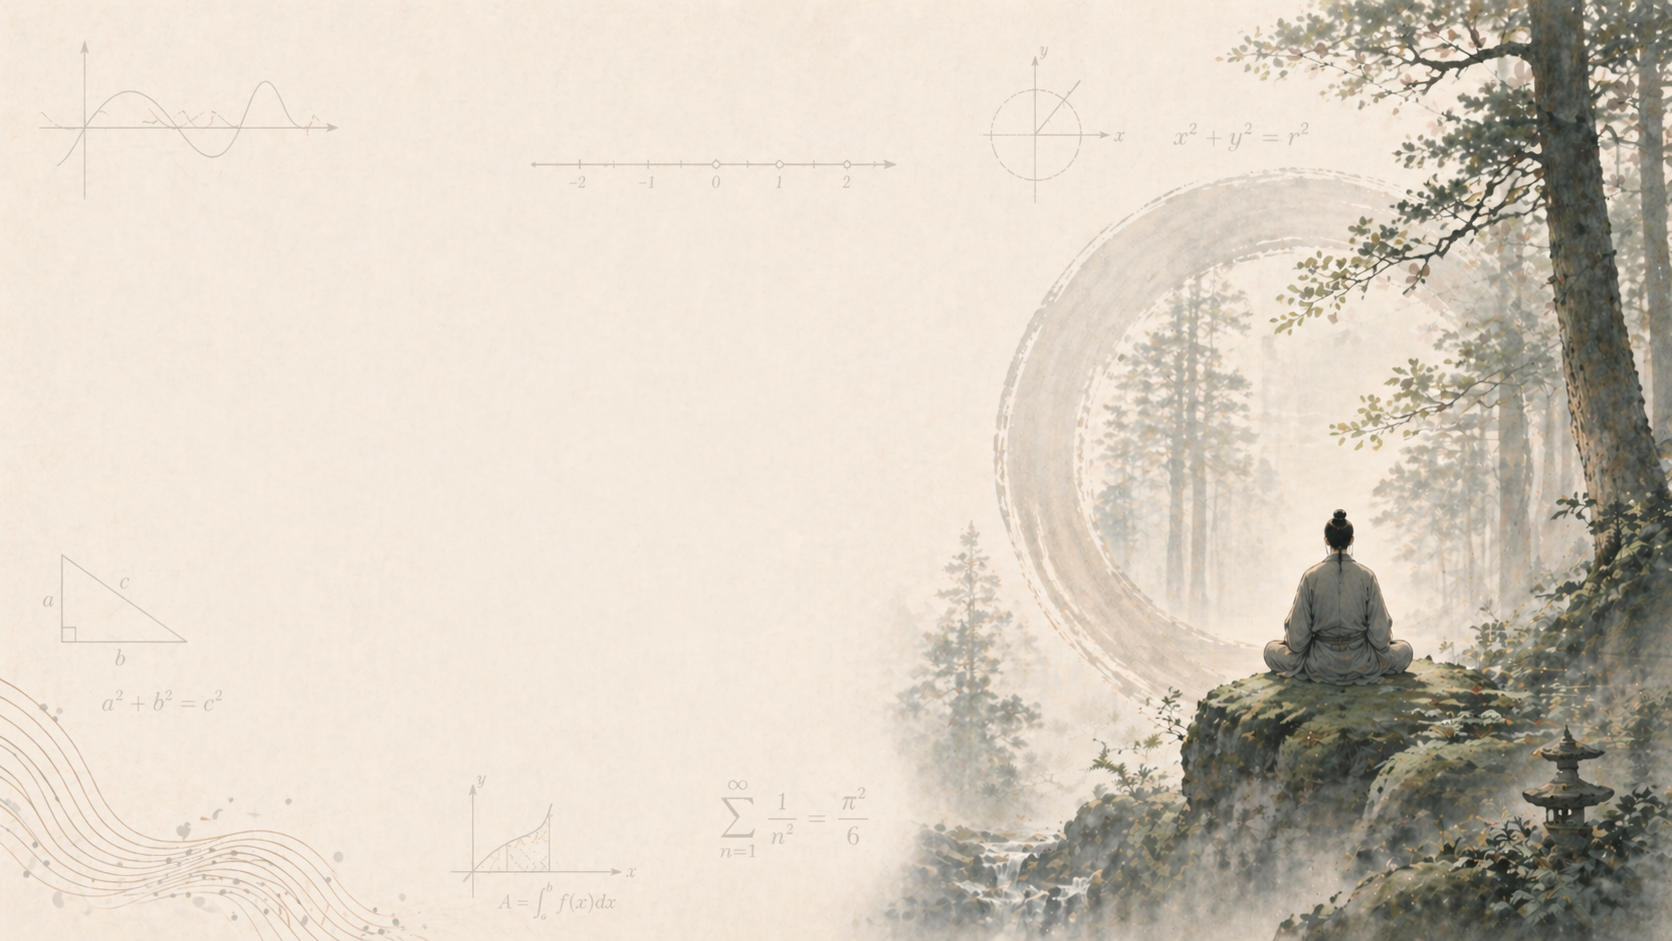
\includegraphics[width=\paperwidth,height=\paperheight,keepaspectratio=false]{chapter_03_bg_07.png}%
}
% =============================================================================
% SUMMARY
% =============================================================================
\section{Summary}

% --- Summary: Build 1/4 ---
\begin{frame}{Summary}
  \begin{hlbox}
    \textbf{Key takeaways from this section:}
    \begin{itemize}
      \item \alert{Def. 3.15:} $s_n \to \pm\infty$ defined for divergent sequences
    \end{itemize}
  \end{hlbox}

  \note{
    Let us recap. We started by formalising what it means for a
    real sequence to diverge to plus or minus infinity. The arrow
    notation now applies in this extended sense, while ordinary
    convergence is unchanged.
  }
\end{frame}

% --- Summary: Build 2/4 ---
\begin{frame}{Summary}
  \begin{hlbox}
    \textbf{Key takeaways from this section:}
    \begin{itemize}
      \item \alert{Def. 3.15:} $s_n \to \pm\infty$ defined for divergent sequences
      \item \alert{Def. 3.16:} $s^* = \limsup s_n = \sup E$, $s_* = \liminf s_n = \inf E$, where $E$ = subsequential limits in $[-\infty,+\infty]$
    \end{itemize}
  \end{hlbox}

  \note{
    We then collected all the subsequential limits, in the
    extended real line, into a single set "E", and defined the
    upper limit as the supremum of "E" and the lower limit as the
    infimum. Crucially, these always exist for any real sequence,
    even one with no ordinary limit.
  }
\end{frame}

% --- Summary: Build 3/4 ---
\begin{frame}{Summary}
  \begin{hlbox}
    \textbf{Key takeaways from this section:}
    \begin{itemize}
      \item \alert{Def. 3.15:} $s_n \to \pm\infty$ defined for divergent sequences
      \item \alert{Def. 3.16:} $s^* = \limsup s_n = \sup E$, $s_* = \liminf s_n = \inf E$, where $E$ = subsequential limits in $[-\infty,+\infty]$
      \item \alert{Thm. 3.17:} $s^*$ is the \emph{unique} number that lies in $E$ and beyond which the tail does not return
    \end{itemize}
  \end{hlbox}

  \note{
    Theorem 3.17 characterised the upper limit by two properties:
    it is itself a subsequential limit, and the sequence
    eventually stays below any value larger than it. These two
    properties pin down "s" star uniquely. The lower limit is
    characterised symmetrically.
  }
\end{frame}

% --- Summary: Build 4/4 ---
\begin{frame}{Summary}
  \begin{hlbox}
    \textbf{Key takeaways from this section:}
    \begin{itemize}
      \item \alert{Def. 3.15:} $s_n \to \pm\infty$ defined for divergent sequences
      \item \alert{Def. 3.16:} $s^* = \limsup s_n = \sup E$, $s_* = \liminf s_n = \inf E$, where $E$ = subsequential limits in $[-\infty,+\infty]$
      \item \alert{Thm. 3.17:} $s^*$ is the \emph{unique} number that lies in $E$ and beyond which the tail does not return
      \item \alert{Convergence criterion:} $\lim s_n = s \iff \limsup s_n = \liminf s_n = s$
      \item \alert{Thm. 3.19:} $s_n \leq t_n$ eventually $\Longrightarrow$ inequalities for $\limsup$ and $\liminf$
    \end{itemize}
  \end{hlbox}

  \note{
    The most practical takeaway is the convergence criterion from
    Example 3.18 part "c": the ordinary limit exists if and only
    if the upper and lower limits agree. We also recorded the
    comparison theorem 3.19, which says that order between two
    sequences is preserved by their upper and lower limits.
  }
\end{frame}

% --- Coming up next ---
\begin{frame}{Coming Up Next}
  \begin{hlbox}
    \textbf{Next section: Some Special Sequences}
    \begin{itemize}
      \item Concrete sequences whose limits we can compute
      \item $n^p$, $p^n$, $n^{1/n}$, and friends
      \item Tools we will reuse for series and analysis
    \end{itemize}
  \end{hlbox}

  \note{
    Coming up next is a short interlude on some special
    sequences. We work out the limits of a few concrete
    expressions: "n" to the power "p", "p" to the "n", and the
    "n"-th root of "n", among others. These are workhorse facts
    that we will reuse throughout the rest of the book,
    especially in the root and ratio tests for series later in
    this chapter, where the upper and lower limits we just
    introduced will play a starring role. See you in the next
    section.
  }
\end{frame}
}

\end{document}
